\section{Operações de remoção}

\begin{frame}[fragile]{Remoção do final e limpeza}

    \begin{itemize}
        \item A remoção do final do vetor tem complexidade $O(1)$

        \item O procedimento é simples: basta decrementar o campo \rawcode{size}

        \item Observe que não é necessário modificar ou alterar o valor do
        último elemento

        \item Embora o valor permaneça inalterado na memória, ele se torna inacessível

        \item A tentativa de remoção de elemento em um vetor vazio constitui um erro, o qual
            deve ser tratado

        \item A função \rawcode{clear()} é semelhante, com a única diferença que o campo
        \rawcode{size} é zerado
    \end{itemize}

\end{frame}

\begin{frame}[fragile]{Visualização da remoção ao final}

    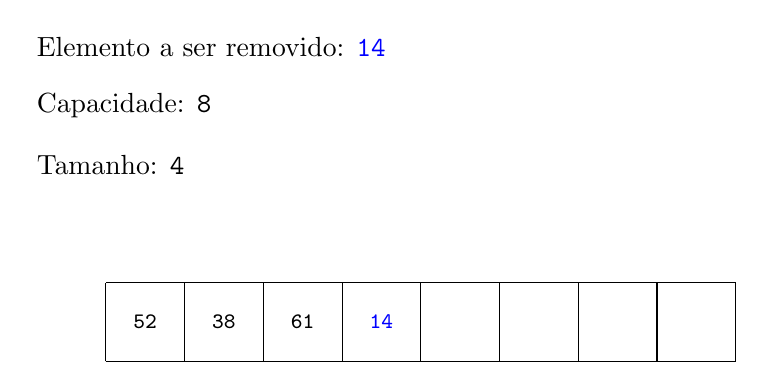
\begin{tikzpicture}
        \node[anchor=west] at (0, 4) {Elemento a ser removido: \texttt{\textcolor{blue}{14}}};
        \node[anchor=west] at (0, 3.25) {Capacidade: \texttt{\textcolor{black}{8}}};
        \node[anchor=west] at (0, 2.5) {Tamanho: \texttt{\textcolor{black}{4}}};
        \draw (1,0) grid (9,1);

        \node at (1.5,0.5) {\footnotesize \texttt{52}};
        \node at (2.5,0.5) {\footnotesize \texttt{38}};
        \node at (3.5,0.5) {\footnotesize \texttt{61}};
        \node at (4.5,0.5) {\footnotesize \texttt{\textcolor{blue}{14}}};
    \end{tikzpicture}

\end{frame}

\begin{frame}[fragile]{Visualização da remoção ao final}

    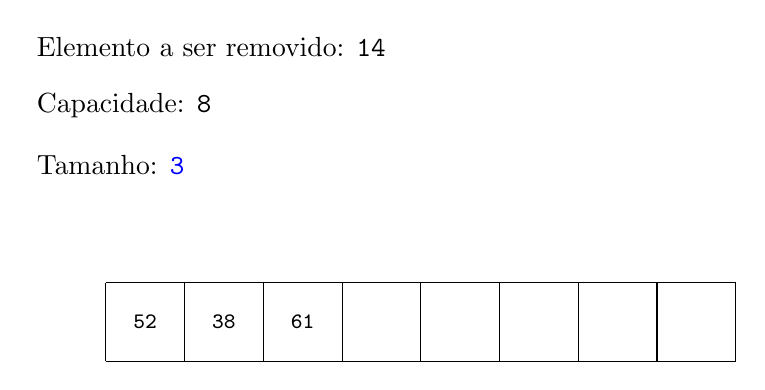
\begin{tikzpicture}
        \node[anchor=west] at (0, 4) {Elemento a ser removido: \texttt{\textcolor{black}{14}}};
        \node[anchor=west] at (0, 3.25) {Capacidade: \texttt{\textcolor{black}{8}}};
        \node[anchor=west] at (0, 2.5) {Tamanho: \texttt{\textcolor{blue}{3}}};
        \draw (1,0) grid (9,1);

        \node at (1.5,0.5) {\footnotesize \texttt{52}};
        \node at (2.5,0.5) {\footnotesize \texttt{38}};
        \node at (3.5,0.5) {\footnotesize \texttt{61}};
        \node at (4.5,0.5) {\footnotesize \texttt{}};
    \end{tikzpicture}

\end{frame}


\begin{frame}[fragile]{Implementação das funções \rawcode{pop\_back()} e \rawcode{clear()}}
    \inputsnippet{c}{108}{128}{codes/vector_adt.c}
\end{frame}

\begin{frame}[fragile]{Remoção em posição arbitrária}

    \begin{itemize}
        \item Assim como na inserção, a remoção em posição arbitrária tem complexidade
        $O(N)$

        \item Novamente o deslocamento é necessário, mas em sentido oposto

        \item Os elementos à direita da posição indicada devem ser deslocados uma posição para a
            esquerda

        \item O campo \rawcode{size} deve ser atualizado

        \item Constitui um erro remover um elemento de uma posição inválida ou de um vetor
        vazio
    \end{itemize}

\end{frame}

\begin{frame}[fragile]{Visualização da remoção em posição arbitrária}

    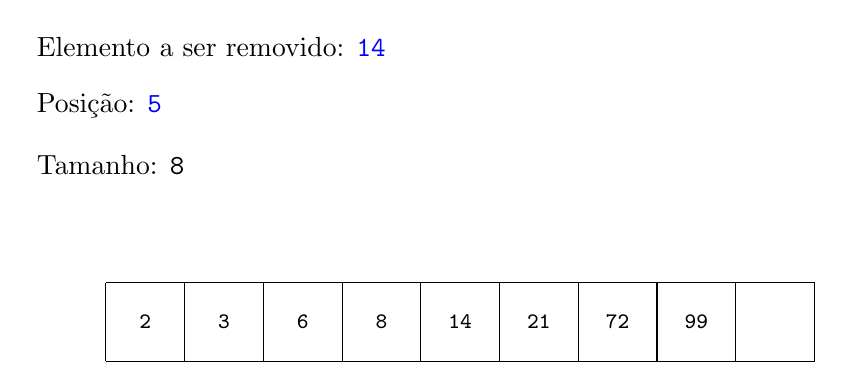
\begin{tikzpicture}
        \node[anchor=west] at (0, 4) {Elemento a ser removido: \texttt{\textcolor{blue}{14}}};
        \node[anchor=west] at (0, 3.25) {Posição: \texttt{\textcolor{blue}{5}}};
        \node[anchor=west] at (0, 2.5) {Tamanho: \texttt{\textcolor{black}{8}}};
        \draw (1,0) grid (10,1);

        \node at (1.5,0.5) {\footnotesize \texttt{2}};
        \node at (2.5,0.5) {\footnotesize \texttt{3}};
        \node at (3.5,0.5) {\footnotesize \texttt{6}};
        \node at (4.5,0.5) {\footnotesize \texttt{8}};
        \node at (5.5,0.5) {\footnotesize \texttt{14}};
        \node at (6.5,0.5) {\footnotesize \texttt{21}};
        \node at (7.5,0.5) {\footnotesize \texttt{72}};
        \node at (8.5,0.5) {\footnotesize \texttt{99}};
    \end{tikzpicture}

\end{frame}

\begin{frame}[fragile]{Visualização da remoção em posição arbitrária}

    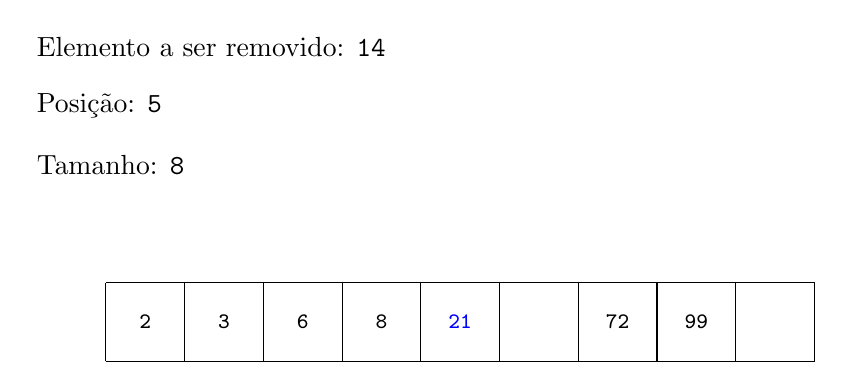
\begin{tikzpicture}
        \node[anchor=west] at (0, 4) {Elemento a ser removido: \texttt{\textcolor{black}{14}}};
        \node[anchor=west] at (0, 3.25) {Posição: \texttt{\textcolor{black}{5}}};
        \node[anchor=west] at (0, 2.5) {Tamanho: \texttt{\textcolor{black}{8}}};
        \draw (1,0) grid (10,1);

        \node at (1.5,0.5) {\footnotesize \texttt{2}};
        \node at (2.5,0.5) {\footnotesize \texttt{3}};
        \node at (3.5,0.5) {\footnotesize \texttt{6}};
        \node at (4.5,0.5) {\footnotesize \texttt{8}};
        \node at (5.5,0.5) {\footnotesize \texttt{\textcolor{blue}{21}}};
        \node at (6.5,0.5) {\footnotesize \texttt{}};
        \node at (7.5,0.5) {\footnotesize \texttt{72}};
        \node at (8.5,0.5) {\footnotesize \texttt{99}};
    \end{tikzpicture}

\end{frame}

\begin{frame}[fragile]{Visualização da remoção em posição arbitrária}

    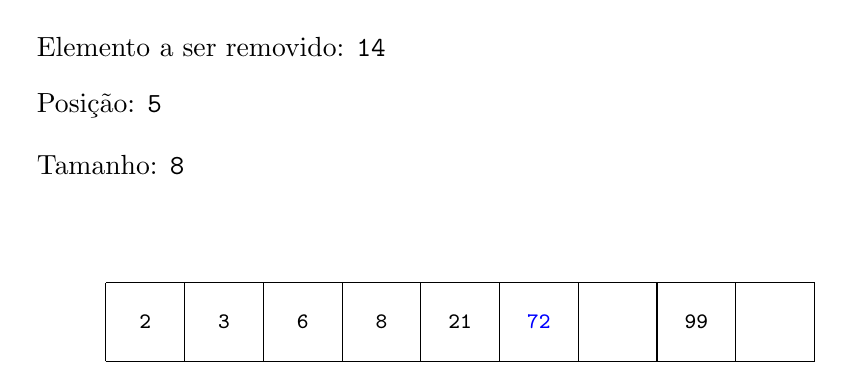
\begin{tikzpicture}
        \node[anchor=west] at (0, 4) {Elemento a ser removido: \texttt{\textcolor{black}{14}}};
        \node[anchor=west] at (0, 3.25) {Posição: \texttt{\textcolor{black}{5}}};
        \node[anchor=west] at (0, 2.5) {Tamanho: \texttt{\textcolor{black}{8}}};
        \draw (1,0) grid (10,1);

        \node at (1.5,0.5) {\footnotesize \texttt{2}};
        \node at (2.5,0.5) {\footnotesize \texttt{3}};
        \node at (3.5,0.5) {\footnotesize \texttt{6}};
        \node at (4.5,0.5) {\footnotesize \texttt{8}};
        \node at (5.5,0.5) {\footnotesize \texttt{\textcolor{black}{21}}};
        \node at (6.5,0.5) {\footnotesize \texttt{\textcolor{blue}{72}}};
        \node at (7.5,0.5) {\footnotesize \texttt{}};
        \node at (8.5,0.5) {\footnotesize \texttt{99}};
    \end{tikzpicture}

\end{frame}

\begin{frame}[fragile]{Visualização da remoção em posição arbitrária}

    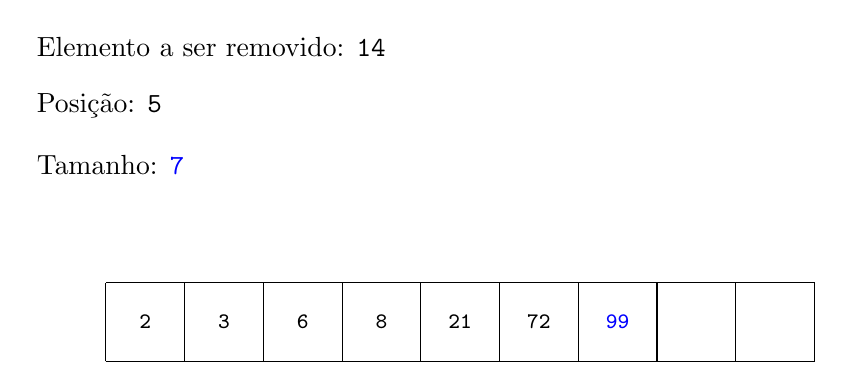
\begin{tikzpicture}
        \node[anchor=west] at (0, 4) {Elemento a ser removido: \texttt{\textcolor{black}{14}}};
        \node[anchor=west] at (0, 3.25) {Posição: \texttt{\textcolor{black}{5}}};
        \node[anchor=west] at (0, 2.5) {Tamanho: \texttt{\textcolor{blue}{7}}};
        \draw (1,0) grid (10,1);

        \node at (1.5,0.5) {\footnotesize \texttt{2}};
        \node at (2.5,0.5) {\footnotesize \texttt{3}};
        \node at (3.5,0.5) {\footnotesize \texttt{6}};
        \node at (4.5,0.5) {\footnotesize \texttt{8}};
        \node at (5.5,0.5) {\footnotesize \texttt{\textcolor{black}{21}}};
        \node at (6.5,0.5) {\footnotesize \texttt{\textcolor{black}{72}}};
        \node at (7.5,0.5) {\footnotesize \texttt{\textcolor{blue}{99}}};
    \end{tikzpicture}

\end{frame}


\begin{frame}[fragile]{Implementação da função \rawcode{pop}}
    \inputsnippet{c}{130}{150}{codes/vector_adt.c}
\end{frame}

\begin{frame}[fragile]{Exemplo de remoção em posição arbitrária}
    \inputsnippet{c}{1}{21}{codes/passageiros2.c}
\end{frame}

\begin{frame}[fragile]{Exemplo de remoção em posição arbitrária}
    \inputsnippet{c}{23}{43}{codes/passageiros2.c}
\end{frame}

\begin{frame}[fragile]{Exemplo de remoção em posição arbitrária}
    \inputsnippet{c}{44}{64}{codes/passageiros2.c}
\end{frame}

\begin{frame}[fragile]{Exemplo de remoção em posição arbitrária}
    \inputsnippet{c}{65}{85}{codes/passageiros2.c}
\end{frame}

